\lhead{\emph{\ChapterFour{}}}
\lstset{
   language=Javascript
}

Antes que nada, se debe crear una instancia del navegador CasperJS, incorporando la librería \textit{casper} y pasando las opciones de creación como argumento.

\begin{center}
\begin{minipage}{\linewidth}
% \label{fig:code01}
\begin{lstlisting}[caption=Creación del navegador CasperJS.]
var casper = require('casper').create({
//  verbose: true,
  logLevel: "debug"
});
\end{lstlisting}
\end{minipage}
\end{center}



\todo{
\begin{codigo}
definir entorno de codigo
\end{codigo}
}

En este caso se le pasa el argumento \textit{verbose} para indicar que se desea que muestre mensajes informativos al realizar las acciones que se le pasen, mientras que el argumento \textit{logLevel} sirve para especificar el detalle que precisamos de esos mensajes. %(Fig. \ref{fig:code01}).

\begin{center}
\begin{minipage}{\linewidth}
\begin{lstlisting}[caption=Estructuras de datos para la navegación por la página.]
// Enlaces hacia las paginas de los TFGs.
var links = [];
// Offset navegado hasta el momento en el catalogo de TFGs.
var offset = 0;
\end{lstlisting}
\end{minipage}
\end{center}

El navegador obtendrá los enlaces a cada página individual de TFG, los cuales deberá mantener en memoria hasta la finalización de la ejecución del programa de extracción de datos.
Es por ello que se define la variable \textit{enlaces} que los contendrá. Por otra parte, al realizar el paginado se debe conocer la posición del navegador de manera inmediata, por lo que se mantiene y actualiza en la variable \textit{offset}. %(Fig. \ref{fig:code02}).

\begin{center}
\begin{minipage}{\linewidth}
\begin{lstlisting}[caption=Estructuras de datos para las características de cada TFG.]
var titles = [];
var descriptions = [];
var tags = [];
\end{lstlisting}
\end{minipage}
\end{center}

Las características que se han tomado como relevantes en la primera aproximación han sido el título, la descripción y las etiquetas que se han dado a cada TFG en el repositorio. Estas se mantendrán en variables separadas. %(Fig. \ref{fig:code03}).

\begin{center}
\begin{minipage}{\linewidth}
\begin{lstlisting}[caption=Función de obtención de enlaces individuales.]
// En cualquier pagina de TFGs recientes de un grado,
// obtener los enlaces a las paginas de los TFGs.
function scrapeLinks() {
    var links = $('li.ds-artifact-item a');
    return Array.prototype.map.call(links, function(e) {
        return e.getAttribute('href');
    });
}
\end{lstlisting}
\end{minipage}
\end{center}

Durante la paginación, cada una de las páginas muestra enlaces individuales hacia cada uno de los Trabajos de Fin de Grado. Para ello, estando el navegador en cualquier página del catálogo, obtenemos los elementos \textit{href} y con ellos todos los enlaces de la vista actual. %(Fig. \ref{fig:code04}).

\begin{center}
\begin{minipage}{\linewidth}
\begin{lstlisting}[caption=Función de paginado.]
// Estando en el catalogo, obtiene el enlace a
// la siguiente pagina del catalogo si la hay.
function scrapeNextPageLink(){
  if ($('.next.pull-right.disabled').length > 0) return null;
  return $('a.next-page-link')[0].href;
}
\end{lstlisting}
\end{minipage}
\end{center}

Durante la paginación, se debe conocer si existe una página subsecuente a aquélla en la que se encuentra el navegador actualmente. Para ello inspeccionamos si el botón que permite paginar a la siguiente página está bloqueado en la vista. De ser este el caso, nos encontramos en la última página. De otro modo, conseguimos el nuevo enlace del elemento de paginación. %(Fig. \ref{fig:code05}).

\begin{center}
\begin{minipage}{\linewidth}
\begin{lstlisting}[caption=Función de obtención de todos los enlaces de TFG.]
/**
* Obtiene todos los enlaces de los TFGs de un Grado.
* Se presupone que Casper se encuentra en
* la primera pagina de TFGs recientes del Grado.
*/
function casperLinksOnThisBachelor(){
    var newLinks = casper.evaluate(scrapeLinks);
    links = links.concat(newLinks);
    var nextLink = casper.evaluate(scrapeNextPageLink);

    casper.echo('nextLink: ' + nextLink);
    if (nextLink) {
        // casper.thenClick(nextLink);
        casper.thenOpen(nextLink);
        casper.then(casperLinksOnThisBachelor);
    } else {
        casper.echo("END");
    }
}
\end{lstlisting}
\end{minipage}
\end{center}

Aplicamos las anteriores funciones en lo que viene a ser el bucle principal del programa, una función recursiva que se detiene cuando el navegador ha llegado a la última página.

\begin{center}
\begin{figure}[!ht]
  \caption{Vista en la que se muestran los metadatos de un TFG.}
  \label{fig:metadata_view}
  \centering
    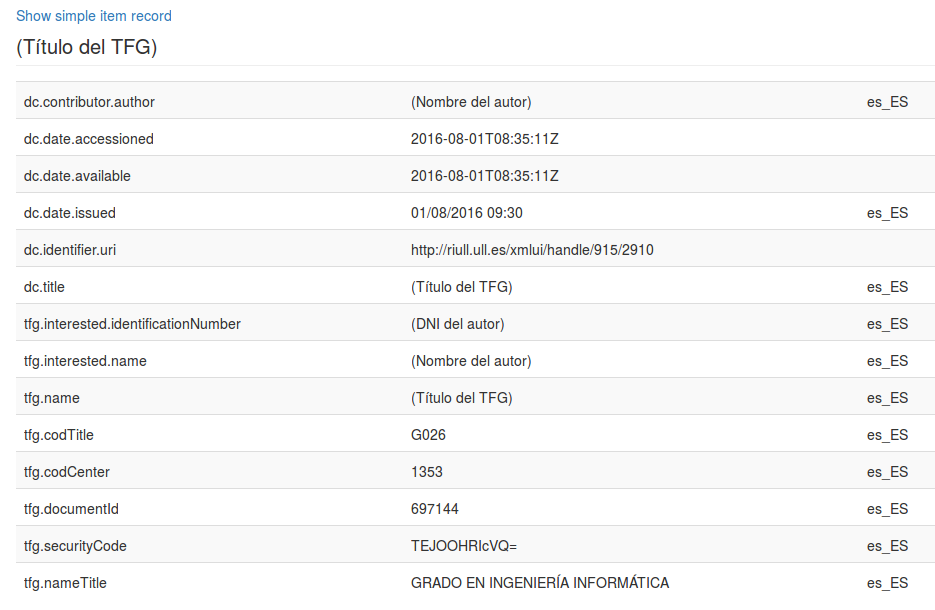
\includegraphics[width=0.8\textwidth]{Images/metadata_view}
\end{figure}
\end{center}

\begin{center}
\begin{minipage}{\linewidth}
\begin{lstlisting}[caption=Función de obtención de metadato por nombre de etiqueta.]
// En una pagina del TFG, obtener el valor del campo 'str' (si lo hay).
function scrapePageValue(str){
    var datum = $('td.label-cell:contains(' + str + ') + td')[0].innerHTML;
    if (datum === null || datum === undefined || datum === "")
        datum = "---";
    return datum;
}
\end{lstlisting}
\end{minipage}
\end{center}

Esta función se basa en la vista de la página para obtener el texto perteneciente a una etiqueta. Por ejemplo, para el caso de la Fig.\ref{fig:metadata_view}, si se le pasa \texttt{author} obtendrá \texttt{(Nombre del autor)}.

% En caso de que no exista, la función devolverá una cadena estándar (en este caso "\texttt{---}") para evitar romper el flujo del programa.

\begin{center}
\begin{minipage}{\linewidth}
\begin{lstlisting}[caption=Función de obtención de metadatos por nombre de etiqueta similar.]
// En una pagina del TFG, obtener el valor de varios campos 'str' (si los hay).
function scrapePageValues(str){
    var data = $('td.label-cell:contains(' + str + ') + td');
    var data2 = [];
    for (var i = 0; i < data.length; i++){
      data2.push(data[i].innerHTML);
    }
    if (data2.length < 1) data2.push("---");
    return data2;
}
\end{lstlisting}
\end{minipage}
\end{center}

Definimos además una función similar a la anterior, con la diferencia de que inspecciona la página para encontrar múltiples datos definidos bajo el mismo nombre. Esto es importante dado que existen metadatos que están definidos bajo campos de mismo nombre, como alternativa a enumerar los distintos valores que toma cierto...

\begin{center}
\begin{minipage}{\linewidth}
\begin{lstlisting}[caption=Función de concatenación de enlace.]
function completeLink(currentValue, index, array){
  return 'http://riull.ull.es'.concat(currentValue).concat('?show=full');
}
\end{lstlisting}
\end{minipage}
\end{center}

% Uno de los problemas fue la imposibilidad de realizar una recurrencia sin blabla, por eso se recurrió a crear una función externa

\begin{center}
\begin{minipage}{\linewidth}
\begin{lstlisting}[caption=Función tipo que permite la recurrencia con CasperJS.]
function functionOutsideLoop(){
  links.concat(casper.evaluate(scrapeLinks));
}
\end{lstlisting}
\end{minipage}
\end{center}
